\chapter{Proposed Solution}

This chapter presents the proposed solution for BK-MInD, a Multimodal Retrieval-Augmented Generation (MRAG) system designed to process and retrieve information from diverse HCMUT educational materials. The chapter first justifies the selection of RAG as the core architectural paradigm over alternative approaches, then presents the rationale for choosing the three key technology components. The system architecture is described across four perspectives: a high-level overview, the data processing and dual-pathway embedding pipelines, the retrieval and generation flow, and the security design. Experimental evidence supporting retrieval architecture decisions is provided, and the chapter concludes with the technical requirements for deployment.

\section{Justification for Retrieval-Augmented Generation}

While LLMs possess remarkable generative capabilities, they suffer from inherent limitations such as knowledge cutoffs, hallucinations, and a lack of access to proprietary data. To address these issues, several methodologies exist. This section analyzes alternative approaches — Fine-Tuning, Semantic Search, Prompt Engineering, and Domain-Specific Pre-training — and justifies the selection of RAG as the superior architectural choice for this project.

\subsection{Comparative Analysis of Alternatives}

\textbf{RAG vs. Fine-Tuning}
Fine-tuning involves retraining a pre-trained LLM on a specific dataset to adjust its internal parameters (weights). While this method tailors the model to a specific domain style, it was rejected for the following reasons:

\begin{itemize}
    \item \textbf{Static Knowledge Base:} Fine-tuned models immediately become outdated upon training completion. Updating the knowledge requires a computationally expensive retraining process. In contrast, RAG allows for \textit{dynamic updates} - simply adding a document to the database makes it immediately retrievable without modifying the model weights.
    \item \textbf{Hallucination Risk:} Fine-tuning increases the probability of the model adopting a specific tone, but it does not guarantee factual accuracy. The model can still hallucinate information effectively. RAG mitigates this by grounding the generation in retrieved evidence.
    \item \textbf{Explainability:} A fine-tuned model outputs an answer based on ``black box'' internal weights. RAG provides citation and source attribution (retrieved chunks), which is critical for verifying accuracy in our application.
\end{itemize}

\textbf{RAG vs. Prompt Engineering (Context Stuffing)}
Prompt engineering involves optimizing the textual input to guide the LLM's output, often by manually pasting context. While simple, it is insufficient for our scale:

\begin{itemize}
    \item \textbf{Context Window Limitations:} Although context windows are growing (e.g., 128k tokens), it is infeasible to pass an entire corpus (e.g., 50,000 documents) into a single prompt. RAG acts as a filter, selecting only the most relevant snippets to fit within the model's constraints.
    \item \textbf{Performance Degradation:} Studies show that as the context length increases, the model's ability to reason over the data (``Lost in the Middle'' phenomenon) decreases. RAG ensures the model focuses only on highly relevant, condensed information.
\end{itemize}

\textbf{RAG vs. Semantic Search (Traditional Information Retrieval)}
Semantic search utilizes Vector Databases to retrieve documents based on meaning rather than keywords. However, it functions solely as a retrieval engine, not a generation engine.

\begin{itemize}
    \item \textbf{Synthesis vs. Retrieval:} Semantic search returns a list of document links or snippets. The user is then forced to read and synthesize the answer manually. RAG automates this cognitive load by employing the LLM to read the retrieved documents and generate a coherent, natural language answer.
    \item \textbf{Completeness:} A user's query might require synthesizing information from three different documents. Semantic search provides the three documents; RAG provides the unified answer derived from them.
\end{itemize}

\textbf{RAG vs. Domain-Specific Pre-training}
Pre-training involves training a model from scratch or continuing pre-training on a massive domain-specific corpus.

\begin{itemize}
    \item \textbf{Computational Cost:} This approach is prohibitively expensive, requiring massive GPU clusters and weeks of training time.
    \item \textbf{Flexibility:} Like fine-tuning, a pre-trained model fails in dynamic environments where data changes daily. RAG decouples the \textit{reasoning engine} (the LLM) from the \textit{knowledge base} (the Vector Database), allowing us to swap or update the knowledge base instantly without touching the neural network.
\end{itemize}

\subsection{Summary of Trade-offs}

The following table summarizes the key architectural decisions that led to the adoption of RAG.

\begin{table}[H]
\centering
\caption{Comparison of RAG against alternative LLM enhancement strategies}
\label{tab:rag_comparison}
\scalebox{0.8}{
\begin{tabular}{lcccc}
\toprule
\textbf{Feature} & \textbf{RAG (Ours)} & \textbf{Fine-Tuning} & \textbf{Prompt Engineering} & \textbf{Semantic Search} \\ \midrule
\textbf{Knowledge Update} & \textit{Real-time (Dynamic)} & Slow (Retraining) & Manual & Real-time \\
\textbf{Hallucination Risk} & Low (Grounded) & High & Medium & N/A (No Generation) \\
\textbf{Context Capacity} & Infinite (via Retrieval) & Limited by Training & Limited by Window & Infinite \\
\textbf{Computational Cost} & Low (Inference only) & High (Training) & Very Low & Low \\
\textbf{Answer Synthesis} & \textbf{Yes} & Yes & Yes & \textbf{No} \\ \bottomrule
\end{tabular}
}
\end{table}

\textbf{Conclusion:}
RAG is chosen because it offers the optimal balance of accuracy, cost-efficiency, and dynamic adaptability. It leverages the reasoning power of pre-trained LLMs while overcoming their memory limitations through external retrieval, making it the most suitable architecture for a document-based Question Answering system.

\section{Technology Selection}

Selecting the right technology stack is critical to the performance, maintainability, and scalability of the BK-MInD system. This section justifies the choice of React for the frontend, FastAPI for the backend, and Qdrant as the cloud vector database — three components that together provide an optimized foundation for a multimodal educational RAG application. Each selection is grounded in a direct comparison with primary alternatives, demonstrating superiority across the key criteria of performance, developer experience, and architectural fit.

\subsection{Frontend: React}

The frontend is the face of the application, defining the user's entire interactive experience with the multimodal output of the RAG system. The choice of a modern JavaScript framework is therefore essential for building a rich, responsive, and maintainable user interface.

After analyzing the leading frameworks, React is the recommended choice. This decision is based on four key pillars:
\begin{itemize}
    \item \textbf{Core Architectural Suitability} for the application's specific technical demands.
    \item \textbf{Superior Performance} in managing frequent and complex UI updates.
    \item \textbf{Unmatched Ecosystem and Community Support}, which directly accelerates development and ensures long-term viability.
    \item \textbf{Proven Precedent} in large-scale, complex applications, particularly within the EdTech industry.
\end{itemize}

From now on, we detail the reasoning for this selection, including a direct comparison with the primary alternative, Vue.js.

\textbf{Architecture Suits a Multimodal RAG System}

The architectural principles of React are uniquely suited to the specific challenges of our application. The RAG system will return a heterogeneous mix of data: a streaming text answer, a reference to a page in a PDF, a timestamp in a lecture video, and a relevant diagram.

React's declarative nature, where developers describe what the UI should look like for a given state, allows the team to manage this complexity effectively. Instead of writing complex, imperative code to manually update the DOM for each data type, developers can create distinct, self-contained components for example \texttt{ChatWindow}, \texttt{SourceDocViewer}, \texttt{VideoPlayer}, \texttt{ImageViewer}.

The main application component then simply manages the application's state and declaratively renders the appropriate components based on the API response. This clear separation of concerns is critical for building a robust and maintainable multimodal user interface.

\textbf{Core Advantages and Technical Rationale}

Beyond its perfect fit for our specific data model, React provides foundational advantages in performance and development efficiency.

\textit{Component-Based Architecture}
This is the cornerstone of the selection. The user interface will be a composition of independent, reusable components (as listed above). This modularity simplifies the entire development lifecycle; each component can be built, tested, and maintained in isolation, which is critical for managing the complexity of the application.

\textit{High Performance with the Virtual DOM}
The RAG system will generate text responses and display various media types. React's use of a Virtual Document Object Model (DOM) is a key performance feature. It creates a lightweight in-memory representation of the UI, calculates the most efficient changes (``diffing''), and minimizes direct, costly manipulations of the actual browser DOM. This results in a smooth, responsive user experience, even as the UI updates frequently with new data from the backend.

\textbf{Comparative Analysis: React vs. Vue.js}

While both React and Vue.js utilize a virtual DOM and a component-based architecture, a direct comparison reveals React's significant advantages for a project of this scale.

\textit{Ecosystem, Community, and Talent Pool}
React boasts a significantly larger and more mature ecosystem than Vue.js. This translates into an unparalleled selection of third-party libraries, state management solutions (like Redux and Zustand), UI component kits (e.g., Material-UI, Ant Design), and development tools. For a feature-rich educational application that will require complex UI elements, such as interactive document viewers, data visualization, and chat interfaces, this vast ecosystem is a critical accelerator, reducing the need to build components from scratch.

Furthermore, industry surveys consistently demonstrate React's dominant position. Stack Overflow's 2023 survey showed that 42.87\% of professional developers use React, compared to 17.64\% for Vue.js\footnote{\url{https://survey.stackoverflow.co/2023/\#most-popular-technologies-webframe-prof}}. This larger talent pool is a pragmatic and significant advantage for a university-based project like ours.

\begin{figure}[H]
    \centering
    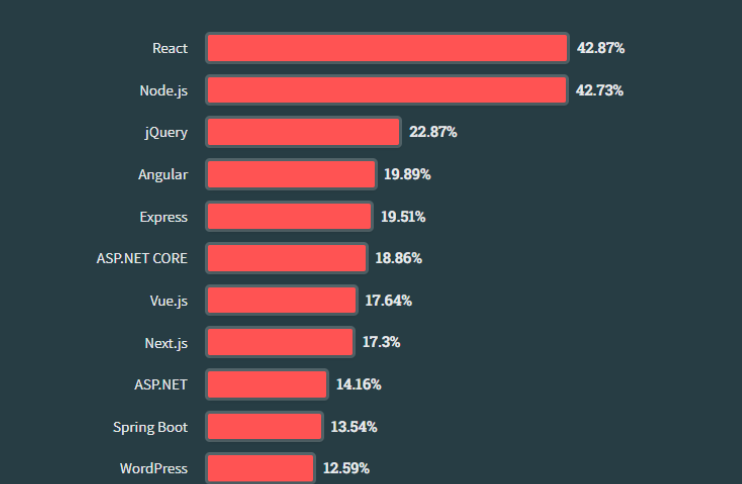
\includegraphics[width=1\textwidth]{img/pdz/33-react-survey.png}
    \caption{Most popular web frameworks and technologies among Professional Developers (Stack Overflow, 2023)}
    \label{fig:react_survey}
\end{figure}

\textit{Scalability and Suitability for Complex Applications}
Both React and Vue.js are capable of building scalable applications. However, React's unopinionated library-based approach provides a crucial flexibility that is often favored for building large-scale, highly complex enterprise applications. This flexibility allows development teams to custom-build their architecture, selecting their own libraries for routing, state management, and data fetching, to create a stack that is perfectly optimized for unique and demanding business logic.

This preference is not merely theoretical; it is validated by the technology stacks of some of the world's largest and most complex web applications:
\begin{itemize}
    \item \textbf{Meta (Facebook \& Instagram)}: As the creator of React, Meta's platforms are its primary case study. The Facebook web app is a quintessential example of a complex, component-driven application, required to manage thousands of individual components, real-time data streaming, and billions of user interactions simultaneously.
    \item \textbf{Netflix}: The Netflix web application relies on React to deliver its high-performance, TV-like user interface. The team chose React to manage the complex state interactions of its UI, enabling them to rapidly iterate, A/B test features, and maintain performance on a wide variety of devices.
    \item \textbf{The New York Times}: To support modern, interactive journalism and a massive, dynamic content library, The New York Times rebuilt its website using React. This allows their development teams to create reusable components that can be shared across the organization, accelerating the development of new features and data visualizations.
\end{itemize}

While Vue is highly capable, React's architecture is battle-tested and proven to be the choice for global teams building applications where complexity and massive scale are the primary concerns.

\subsection{Backend: FastAPI}

The backend is the engine of our AI-driven educational application, responsible for orchestrating every interaction between the user, our data stores, and the core AI models. Our reliance on Python is a strategic imperative, granting us native access to the world's leading AI ecosystem, including libraries like PyTorch, Scikit-learn, and the Hugging Face ecosystem.

Within this ecosystem, the choice of web framework is critical. It is the layer that can either unleash the power of our AI models or become a crippling performance bottleneck. After a detailed analysis of the primary contenders, the mature, ``batteries-included'' Django framework and the modern, high-performance FastAPI, we have concluded that FastAPI is the unequivocally superior choice for this project.

This decision is based on three core pillars:
\begin{itemize}
    \item \textbf{Exceptional Performance}: FastAPI's asynchronous architecture delivers an order-of-magnitude performance improvement over traditional frameworks, which is essential for the I/O-bound nature of a Retrieval-Augmented Generation (RAG) application.
    \item \textbf{Accelerated Developer Experience}: Its modern, type-hint-driven design, featuring automatic data validation and API documentation, drastically reduces boilerplate code and minimizes common errors.
    \item \textbf{Future-Proof Architectural Philosophy}: FastAPI is designed for a modern, microservices-first world, providing the flexibility and scalability required to prevent technical debt and support long-term growth.
\end{itemize}

\textbf{Performance and Asynchronous Processing}

A RAG application is inherently I/O-bound. The server spends most of its time not computing, but waiting: waiting for a query response from the Vector Database, waiting for user data from a relational database, and, most significantly, waiting for the Large Language Model (LLM) API to stream back its generated response.

In a traditional synchronous framework like Django, each of these waiting periods would block an entire worker thread. This means that if 10 users send a query simultaneously, the application needs at least 10 worker threads, each consuming significant memory. This model scales poorly, leading to a rapid increase in server costs and a degradation of user experience under load.

FastAPI solves this problem at its core. It is built on modern Python \texttt{async/await} syntax and the Asynchronous Server Gateway Interface (ASGI) standard. This allows a single process to handle thousands of concurrent connections. When a task starts waiting for an I/O operation (like an LLM call), the server doesn't block; it yields control and serves other requests, returning to the original task only when the data is ready.

\textbf{Real-World Performance Benchmarks}

This architectural difference is not merely theoretical; it is reflected in stark performance metrics from independent, industry-standard benchmarks. According to the highly respected TechEmpower benchmarks, which test hundreds of web frameworks in realistic scenarios, FastAPI's performance is in a different league.

In the Round 22 benchmarks (testing against physical hardware), the Uvicorn server running a basic FastAPI application handled \textbf{12,567 requests per second} in the Multiple Queries test. In contrast, Django on Gunicorn (a standard synchronous setup) handled \textbf{1,623 requests per second}.

This means FastAPI can handle over 8 times the traffic with the same hardware for this common task\footnote{\url{https://www.techempower.com/benchmarks/\#section=data-r22&test=query}}. For our I/O-bound application, this advantage is even more pronounced. The ability to efficiently manage concurrent waiting tasks means we can serve more users simultaneously with lower latency and significantly lower infrastructure costs. This raw performance is essential for delivering the responsive, real-time experience that users expect from an interactive AI assistant.

\textbf{The Superior Developer Experience}

Beyond raw performance, FastAPI is engineered with a laser focus on building APIs, which dramatically improves developer productivity and code quality.

\begin{itemize}
    \item \textbf{Automatic Data Validation \& Serialization}: FastAPI leverages the Pydantic library and Python type hints to provide automatic request validation. This is a game-changer. Developers simply define the expected data structure as a Python class, and FastAPI handles the rest: validating incoming data, returning clear JSON error messages if validation fails, serializing complex data types, and converting data seamlessly. In Django, achieving this requires the Django REST Framework (DRF), which involves writing separate Serializer classes, adding boilerplate and cognitive load.
    \item \textbf{Automatic Interactive API Documentation}: Out of the box, FastAPI generates interactive API documentation based on the OpenAPI standard. As soon as an endpoint is written, a fully functional documentation page is available at \texttt{/docs}, allowing frontend developers and consumers to test endpoints and understand the API without manual effort. This tight feedback loop is invaluable for rapid development.
\end{itemize}

\textbf{Architectural Philosophy and Future-Proofing}

The choice between FastAPI and Django represents a fundamental decision between a modern, microservices-first architecture and a traditional, monolithic one.

Django's philosophy is geared towards building monolithic, full-stack applications with server-rendered templates, an admin panel, and a built-in ORM. These are excellent features for certain projects, but they are less critical for our API-first, decoupled architecture.

FastAPI's lightweight and unopinionated nature makes it a natural fit for building independent, scalable microservices. This allows for a logical separation of concerns. We can develop, deploy, and scale the user authentication service independently from the RAG pipeline service. This modularity offers significant long-term advantages in scalability and maintainability, preventing the need for a costly and disruptive rewrite as the platform grows.

\textbf{Head-to-Head Comparison Matrix}

The following table provides a clear, at-a-glance comparison to justify the selection of FastAPI for our specific application context.

\begin{table}[H]
    \centering
    \caption{FastAPI vs. Django Comparison for RAG Application}
    \label{tab:fastapi_vs_django}
    \scalebox{0.8}{
    \begin{tabular}{p{3cm}p{4.5cm}p{4.5cm}p{6cm}}
        \toprule
        \textbf{Criterion} & \textbf{FastAPI} & \textbf{Django} & \textbf{Justification for RAG Application} \\
        \midrule
        Performance (Req/s) & Very High ($\sim$12,500+) & Moderate ($\sim$1,600) & RAG requires high concurrency for I/O-bound tasks. FastAPI's 8x+ performance is a decisive advantage. \\
        Asynchronous Support & Native, built-in (\texttt{async/await}) & Supported via Channels (adds complexity) & Native async is simpler and more performant for orchestrating LLM and database calls. \\
        API Documentation & Automatic (Swagger UI, ReDoc) & Requires external library (DRF) & Automatic documentation accelerates development, reduces friction, and simplifies API integration. \\
        Data Validation & Built-in via Pydantic Type Hints & Built-in Forms / DRF Serializers & Pydantic is more modern, concise, and integrated, reducing boilerplate and potential errors. \\
        Architectural Fit & Microservices, API-first & Monolithic, full-stack & A microservices approach is inherently more scalable and maintainable for our project's distinct components. \\
        Learning Curve & Low & Moderate to High & A lower learning curve allows for faster onboarding of new developers and contributors. \\
        \bottomrule
    \end{tabular}
    }
\end{table}

\subsection{Cloud Vector Database: Qdrant}

The market for cloud Vector Databases is highly fragmented, with vendors utilizing fundamentally different programming languages, scaling architectures, and index structures. Evaluating their capacity to handle billion-scale multimodal workloads requires a granular architectural analysis of each platform.

\textbf{Multi-Embedding Storage and MaxSim Execution}

The capacity to efficiently ingest, store, and query the multi-embeddings generated by ColPali is a primary differentiator among Vector Databases. While platforms like \textbf{Vespa} and \textbf{Milvus} offer robust native solutions via tensor formalism and unified data types respectively, \textbf{Qdrant} uniquely excels through its decoupling of storage and indexing. Acknowledging that indexing heavy multi-vector payloads via HNSW wastes compute and RAM, Qdrant allows architects to explicitly disable graph construction for these payloads. They are utilized exclusively for in-memory, query-time MaxSim reranking against candidates retrieved via a fast single-vector pass. This architectural brilliance prevents the database from collapsing under graph maintenance during ingestion, ensuring high-speed data loading and significantly reduced RAM overhead.

\begin{table}[H]
    \centering
    \caption{Multi-Vector Storage and MaxSim Implementation}
    \label{tab:multivector_impl}
    \scalebox{0.8}{
    \begin{tabular}{llll}
        \toprule
        \textbf{Platform} & \textbf{Native Storage} & \textbf{MaxSim Implementation} & \textbf{ColQwen Optimization} \\
        \midrule
        Vespa & Yes (Tensor Formalism) & Yes (Float \& Hamming) & Phased retrieval, BQ \\
        Milvus & Yes (Array of Structs) & Yes (MAX\_SIM Metric) & Entity retrieval \\
        \textbf{Qdrant} & \textbf{Yes (Nested Arrays)} & \textbf{Yes (Query-time compute)} & \textbf{Index bypassing (m=0)} \\
        Weaviate & Yes (Multi-vector) & Yes & Jina AI integration \\
        Pinecone & Partial (Metadata) & Yes (Cascading logic) & ConstBERT mapping \\
        \bottomrule
    \end{tabular}
    }
\end{table}

\textbf{Supported Search Mechanisms}

A robust multimodal database must support various search paradigms. All major platforms natively support dense, sparse (keyword), and hybrid search mechanisms. The critical differentiator is the underlying hybrid fusion algorithm. \textbf{Qdrant} stands out by supporting advanced fusion techniques such as Reciprocal Rank Fusion (RRF) and Distribution-Based Score Fusion (DBSF), intelligently balancing the unbounded scoring of BM25 against the normalized bounds of cosine similarity. Furthermore, Qdrant leads the industry in metadata filtering via its highly optimized payload indexing, allowing complex JSON-based logical conditions to intersect with vector search without compromising retrieval speed.

\begin{table}[H]
    \centering
    \caption{Search Mechanism Comparison}
    \label{tab:search_mechanisms}
    \scalebox{0.8}{
    \begin{tabular}{llllll}
        \toprule
        \textbf{Mechanism} & \textbf{Vespa} & \textbf{Milvus} & \textbf{Qdrant} & \textbf{Weaviate} & \textbf{Pinecone} \\
        \midrule
        Keyword / BM25 & Yes (Native) & Yes (Sparse) & Yes (Sparse) & Yes (Inverted) & No \\
        Semantic Dense & Yes & Yes & Yes & Yes & Yes \\
        Hybrid Fusion & RRF, Tensor & Built-in Rankers & \textbf{RRF, DBSF} & Alpha weight & Sparse/Dense \\
        Metadata Filter & Yes & JSON Shred & \textbf{Payload Index} & Yes & High Speed \\
        \bottomrule
    \end{tabular}
    }
\end{table}

\textbf{Scalability, Latency, and Economics}

Transitioning to production demands rigorous evaluation of latency, scalability, and Total Cost of Ownership (TCO). Driven by its \textbf{Rust-based engine}, Qdrant demonstrates exceptional performance, maintaining 30-40 millisecond p95 latencies and sustaining 8,000 to 15,000 QPS, significantly outperforming Go-based alternatives in tail latency. Economically, Qdrant offers a generous perpetual free tier for prototyping and scales cost-effectively via custom sharding and the Raft consensus protocol, whereas enterprise solutions like Milvus and Vespa carry higher base infrastructure costs.

\begin{table}[H]
    \centering
    \caption{Cloud Scalability, Latency, and Economic Efficiency}
    \label{tab:scalability_econ}
    \scalebox{0.8}{
    \begin{tabular}{llllp{4cm}}
        \toprule
        \textbf{Platform} & \textbf{p95 Latency} & \textbf{Throughput} & \textbf{Cost (10M Vec)} & \textbf{Architecture} \\
        \midrule
        \textbf{Qdrant} & \textbf{30-40ms} & \textbf{8k - 15k} & \textbf{\$120 - \$250} & \textbf{Custom Sharding, Raft} \\
        Weaviate & 50-70ms & 3k - 8k & \$150 - \$300 & Sharded Index, K8s \\
        Milvus & 50-80ms & 10k - 20k & \$300 - \$600 & Tiered Storage \\
        Pinecone & Sub-100ms & Auto-scale & \$200 - \$400 & Serverless Pods \\
        Vespa & Sub-100ms & Extreme & Usage-based & Distributed Data Nodes \\
        \bottomrule
    \end{tabular}
    }
\end{table}

\textbf{Developer Experience and Integration}

Developer experience dictates integration speed. While Weaviate offers simplified APIs, it can lack granular configurability. Vespa provides deep tensor control but suffers from an exceptionally steep learning curve. \textbf{Qdrant} strikes the perfect balance. It features straightforward Docker deployments, highly readable Python SDKs, and deep integration with the \texttt{FastEmbed} library. This allows developers to generate dense and sparse embeddings locally without heavy external dependencies, vastly simplifying the creation of multi-vector RAG pipelines.

\textbf{Final Selection and Strategic Recommendation}

\begin{table}[H]
    \centering
    \caption{Holistic Vector Database Comparison Summary}
    \label{tab:holistic_db_comp}
    \scalebox{0.8}{
    \begin{tabular}{llllll}
        \toprule
        \textbf{Feature} & \textbf{Vespa} & \textbf{Milvus} & \textbf{Qdrant} & \textbf{Weaviate} & \textbf{Pinecone} \\
        \midrule
        Core Architecture & Hybrid C++ / Java & Go (K8s) & \textbf{Rust} & Go & SaaS \\
        ColQwen Support & Native Tensor & Array of Structs & \textbf{Index Bypassing} & Multi-vector arrays & Metadata strings \\
        Pricing Model & Usage-based & Tiered Cloud & \textbf{Free Tier + Cloud} & 14-day + Cloud & Free Tier + Pods \\
        Developer Curve & High Complexity & Moderate & \textbf{Low} & Low & Very Low \\
        \bottomrule
    \end{tabular}
    }
\end{table}

After an exhaustive analysis of architectural design, search mechanism breadth, economic efficiency, and specific multi-vector handling capabilities, we have selected \textbf{Qdrant} as the primary cloud Vector Database for the production environment.

\textbf{Strategic Rationale for Selecting Qdrant}:
Qdrant serves as the optimal highly performant alternative for our multimodal RAG architecture. Its architectural decision to bypass HNSW indexing for heavy multi-vector payloads demonstrates a deep understanding of memory economics, ensuring high-speed ingestion and reduced RAM overhead. For our team, Qdrant's native support for late-interaction multi-vector embeddings makes ColQwen integration exceptionally streamlined, while its Rust-powered engine provides the necessary latency and throughput performance for the system.

Having selected the core technology stack (React frontend, FastAPI backend, and Qdrant vector database), the following section presents empirical benchmarks of embedding and retrieval configurations to validate these technology choices and inform the architectural design decisions documented in Section~\ref{sec:system_arch}.

\section{Experiments on Embeddings and Retrieval Methods}

\subsection{Experimental Methodology}

\textbf{Dataset and Computing Environment}
To benchmark the performance of different retrieval architectures, we utilized the \textbf{Microsoft MS MARCO} (Machine Reading Comprehension) dataset\footnote{\url{https://huggingface.co/datasets/microsoft/ms_marco}}. This dataset is a standard benchmark for information retrieval tasks.

Due to computational constraints and to facilitate rapid iterative testing, we curated a representative subset of the data:
\begin{itemize}
    \item \textbf{Corpus Size:} 50,000 documents (reduced from the original $\approx$1 million).
    \item \textbf{Test Queries:} 556 distinct evaluation queries.
    \item \textbf{Hardware Infrastructure:} All experiments were conducted on Google Colab utilizing a single \textbf{Tesla T4 GPU}.
\end{itemize}

\textbf{Scoring Formulations}
Different pipelines utilize distinct mathematical formulations to calculate the relevance score $S(Q, D)$ between a query $Q$ and a document $D$.

\textbf{1. Lexical Scoring (BM25)}

For the sparse retrieval baseline, we employed the BM25 algorithm. This probabilistic model estimates relevance based on term frequency (TF) and inverse document frequency (IDF), normalizing for document length
\begin{equation*}
    \text{Score}_{\text{BM25}}(Q, D) = \sum_{t \in Q} \text{IDF}(t) \cdot \frac{\text{TF}(t, D) \cdot (k_1 + 1)}{\text{TF}(t, D) + k_1 \cdot \left(1 - b + b \cdot \frac{|D|}{\text{avgdl}}\right)}
\end{equation*}
This method focuses on exact keyword matching and is highly effective for queries containing specific identifiers (e.g., proper nouns), though it lacks semantic understanding.

\textbf{2. Semantic Scoring (Dense Retrieval)}

For dense retrieval (e.g., MiniLM, BGE), we encode both query and document into fixed-size vectors ($\vec{V}_Q, \vec{V}_D$) and calculate the Cosine Similarity. This captures semantic meaning beyond exact keyword overlap
\begin{equation*}
    \text{Score}_{\text{Dense}}(Q, D) = \frac{\vec{V}_{Q} \cdot \vec{V}_{D}}{|\vec{V}_{Q}| \cdot |\vec{V}_{D}|}
\end{equation*}
The score range is $[-1, 1]$, representing the semantic proximity in the vector space.

\textbf{3. Late Interaction Scoring (ColBERT/ColQwen)}

Unlike dense retrievers that compress a document into a single vector, the Late Interaction architecture (used in ColBERTv2) encodes queries and documents into bags of embedding vectors. The relevance score is the sum of the maximum similarity (MaxSim) for each query token against all document tokens
\begin{equation*}
    \text{Score}_{\text{MaxSim}}(Q, D) = \sum_{q \in \vec{Q}} \max_{d \in \vec{D}} (\vec{q} \cdot \vec{d})
\end{equation*}
This allows for fine-grained matching, ensuring that specific details in a document are not lost during vector compression.

\textbf{Evaluation Metrics}
To quantitatively assess the pipelines, we adhere to two standard information retrieval metrics:

\begin{enumerate}
    \item \textbf{Recall@k:} Measures the percentage of relevant documents successfully retrieved within the top $k$ results.
    \[
    \text{Recall@k} = \frac{| \{ \text{Relevant Docs} \} \cap \{ \text{Retrieved Top-k} \} |}{| \{ \text{Total Relevant Docs} \} |}
    \]
    \item \textbf{nDCG@k (Normalized Discounted Cumulative Gain):} This metric evaluates the \textit{ranking quality}. It rewards algorithms that place relevant documents at the top of the list.
    \[
    \text{nDCG@k} = \frac{DCG@k}{IDCG@k} \quad \text{where} \quad DCG@k = \sum_{i=1}^{k} \frac{2^{rel_i} - 1}{\log_2(i+1)}
    \]
\end{enumerate}

\subsection{Pipeline Analysis and Results}

\textbf{Important Note on Implementation Status:} The following benchmark results represent experimental evaluations of different retrieval pipeline configurations. However, in the current Phase 2 production deployment, \textbf{reranking is globally disabled} by default (\texttt{SKIP\_RERANKER=true}) for latency optimization. The reranker code is retained in the codebase for fast rollback if needed, but is not invoked during standard search operations. These experimental results are preserved for reference and historical context, but readers should be aware that the production system operates without the reranking stage.

We conducted a comprehensive evaluation of Lexical, Dense, Hybrid, and Reranking pipelines. The aggregate results are presented in Table \ref{tab:results}.

\begin{table}[H]
\centering
\caption[Retrieval Pipeline Performance]{Comparative performance of Retrieval and Reranking pipelines on the MS MARCO subset (50k docs, 556 queries).}
\label{tab:results}
\begin{tabular*}{\textwidth}{@{\extracolsep{\fill}}l l c c r@{}}
\toprule
\textbf{Pipeline Strategy} & \textbf{Model / Configuration} & \textbf{Latency} & \textbf{nDCG@3} & \textbf{Recall@3} \\ \midrule
\multicolumn{5}{l}{\textbf{Baseline Retrievers (No Rerank)}} \\
Sparse & BM25 (rank-bm25) & 3m & 0.2821 & 0.3085 \\
Dense & MiniLM-L6 (Raw) & $\sim$1s & 0.8658 & 0.9125 \\
Dense & \textbf{BGE-Small-en-v1.5} & $\sim$1s & \textbf{0.8855} & \textbf{0.9257} \\ \midrule
\multicolumn{5}{l}{\textbf{Hybrid Retrievers (Reciprocal Rank Fusion)}} \\
Hybrid & BM25 + MiniLM ($k=60$) & $\sim$1s & 0.5786 & 0.6885 \\
Hybrid & BM25 + BGE ($k=60$) & $\sim$1s & 0.5830 & 0.6787 \\ \midrule
\multicolumn{5}{l}{\textbf{Reranking Pipelines (Retrieve + Cross-Encoder)}} \\
Retrieve + Rerank & BM25 + BGE-Large & 1m 43s & 0.4469 & 0.4592 \\
Retrieve + Rerank & MiniLM + BGE-Large & 1m 43s & 0.9196 & 0.9526 \\
Retrieve + Rerank & \textbf{BGE-Small + BGE-Large} & 1m 43s & \textbf{0.9248} & \textbf{0.9598} \\ \midrule
\multicolumn{5}{l}{\textbf{Late Interaction}} \\
Late Interaction & \textbf{ColBERTv2 (RAGatouille)} & 6.5s & \textbf{0.9638} & \textbf{0.9412} \\ \bottomrule
\end{tabular*}
\end{table}

\textbf{Question 1: Is Hybrid Retrieval superior to single-mode retrieval?}
Our experiments demonstrate that Hybrid Retrieval (combining BM25 and Dense vectors via Reciprocal Rank Fusion) offers a significant improvement over purely lexical methods, providing a balanced approach to robustness.

\begin{itemize}
    \item \textbf{Limitations of BM25:} The raw BM25 baseline yielded a low nDCG@3 of $0.2821$. This confirms that the MS MARCO dataset relies heavily on semantic understanding rather than exact keyword matches, causing BM25 to fail when vocabulary mismatches occur.
    \item \textbf{The Hybrid Improvement:} By fusing BM25 with Dense retrieval (Hybrid BGE), the nDCG@3 score improved from $0.2821$ to $0.5830$, representing a \textbf{2.06x improvement} over pure lexical search. However, this remains substantially below the pure dense baseline ($0.8855$), indicating that hybrid retrieval sacrifices some semantic accuracy in exchange for keyword robustness.
    \item \textbf{Significance:} While pure dense models performed exceptionally well on this specific dataset ($0.8855$), relying solely on dense retrieval in production carries the risk of ``semantic hallucination'' (retrieving conceptually similar but factually incorrect documents). Hybrid retrieval mitigates this by anchoring the semantic search with the keyword precision of BM25. It provides a ``safety net'' that ensures documents containing critical entity names are not discarded, making it a more robust strategy for real-world applications where query intent varies.
\end{itemize}

\textbf{Important Note on Generalization}: The experimental results presented above are based on the MS MARCO dataset, a generic domain benchmark for web search contexts. HCMUT lecture materials differ significantly in their characteristics: they contain mathematical notation, domain-specific terminology, structured course hierarchies, and pedagogical content unlike general web documents. Future evaluation should include HCMUT-specific test queries and lecture content to validate whether the retrieved ranking methods (particularly hybrid vs. pure dense) perform equally well for educational domain-specific IR tasks. The generalization of these findings to educational content quality is documented in the Future Plan section (Section 7.4), where HCMUT-specific validation with student cohorts is planned.

\textbf{Question 2: Does the addition of a Reranker significantly improve ranking quality?}
The results strongly support the hypothesis that a two-stage ``Retrieve-then-Rerank'' pipeline outperforms single-stage retrieval, though at a significant latency cost.

\begin{itemize}
    \item \textbf{Architectural Advantage:} We employed Cross-Encoders (specifically \textbf{BAAI/bge-reranker-large}) as the second stage. Unlike bi-encoders, cross-encoders process the query and document simultaneously in the Transformer, capturing deep interaction signals.
    \item \textbf{Performance Gain:} Applying the BGE-Large reranker to the BGE-Small retriever candidates improved nDCG@3 from $0.8855$ to \textbf{0.9248} and Recall@3 from $0.9257$ to \textbf{0.9598}.
    \item \textbf{Latency Trade-off:} We observed that larger rerankers yield better quality but at significantly higher computational cost. The \textbf{bge-reranker-large} consistently outperformed the smaller \textbf{ms-marco-MiniLM-L-12} (e.g., 0.9248 vs 0.9107), but requires approximately \textbf{1 minute 43 seconds} per query (~100x slower than retrieval-only baseline). This latency makes reranking unsuitable for interactive chat applications.
    \item \textbf{Production Decision:} While reranking demonstrates empirical accuracy gains, the BK-MInD Phase 2 production system \textbf{globally disables reranking} (\texttt{SKIP\_RERANKER=true}) by default for interactive latency requirements. The reranker code is retained in the codebase for future evaluation and fast rollback if production requirements change.
\end{itemize}

\textbf{Question 3: Is ColBERT (Late Interaction) the most effective approach?}
Our data indicates that ColBERTv2 provides the highest retrieval quality, surpassing even the best Retrieve-then-Rerank pipelines.

\begin{itemize}
    \item \textbf{Superior Metrics:} ColBERTv2 achieved the highest \textbf{nDCG@3 of 0.9638}, outperforming the best reranking pipeline ($0.9248$).
    \item \textbf{Solving the Information Bottleneck:} Standard two-stage pipelines suffer from a bottleneck: if the first-stage retriever (e.g., BGE-Small) fails to find the relevant document in the top 30 candidates, the Reranker never sees it. ColBERT avoids this by using a ``Late Interaction'' mechanism. It calculates the MaxSim between query tokens and document tokens directly.
    \item \textbf{Granularity:} ColBERT matches at the token level using the MaxSim scoring mechanism described in the methodology section. This allows it to identify a relevant document even if only a small paragraph within it matches the query — a nuance often lost when compressing a whole document into a single vector (Dense Retrieval).
    \item \textbf{Operational Note:} It is worth noting that while ColBERT's retrieval time is efficient ($6.5s$ on GPU), the indexing process is resource-intensive. In our environment, indexing required $\approx35$ minutes on CPU\footnote{Due to FAISS-GPU limitations on the Colab instance, indexing fell back to CPU.} compared to mere seconds/minutes for standard dense models. Despite this setup cost, ColBERT represents the state-of-the-art for retrieval accuracy on this dataset.
\end{itemize}

\section{System Architecture Design}

This section presents the proposed architecture of the BK-MInD MRAG system, organized from a high-level system overview down to specific architectural components for retrieval and security. Implementation details, processing parameters, and deployment specifications are documented in Chapter~6 (Implementation).

\subsection{High-Level Architecture}\label{sec:highlevel_arch}

\begin{figure}[h!]
    \centering
    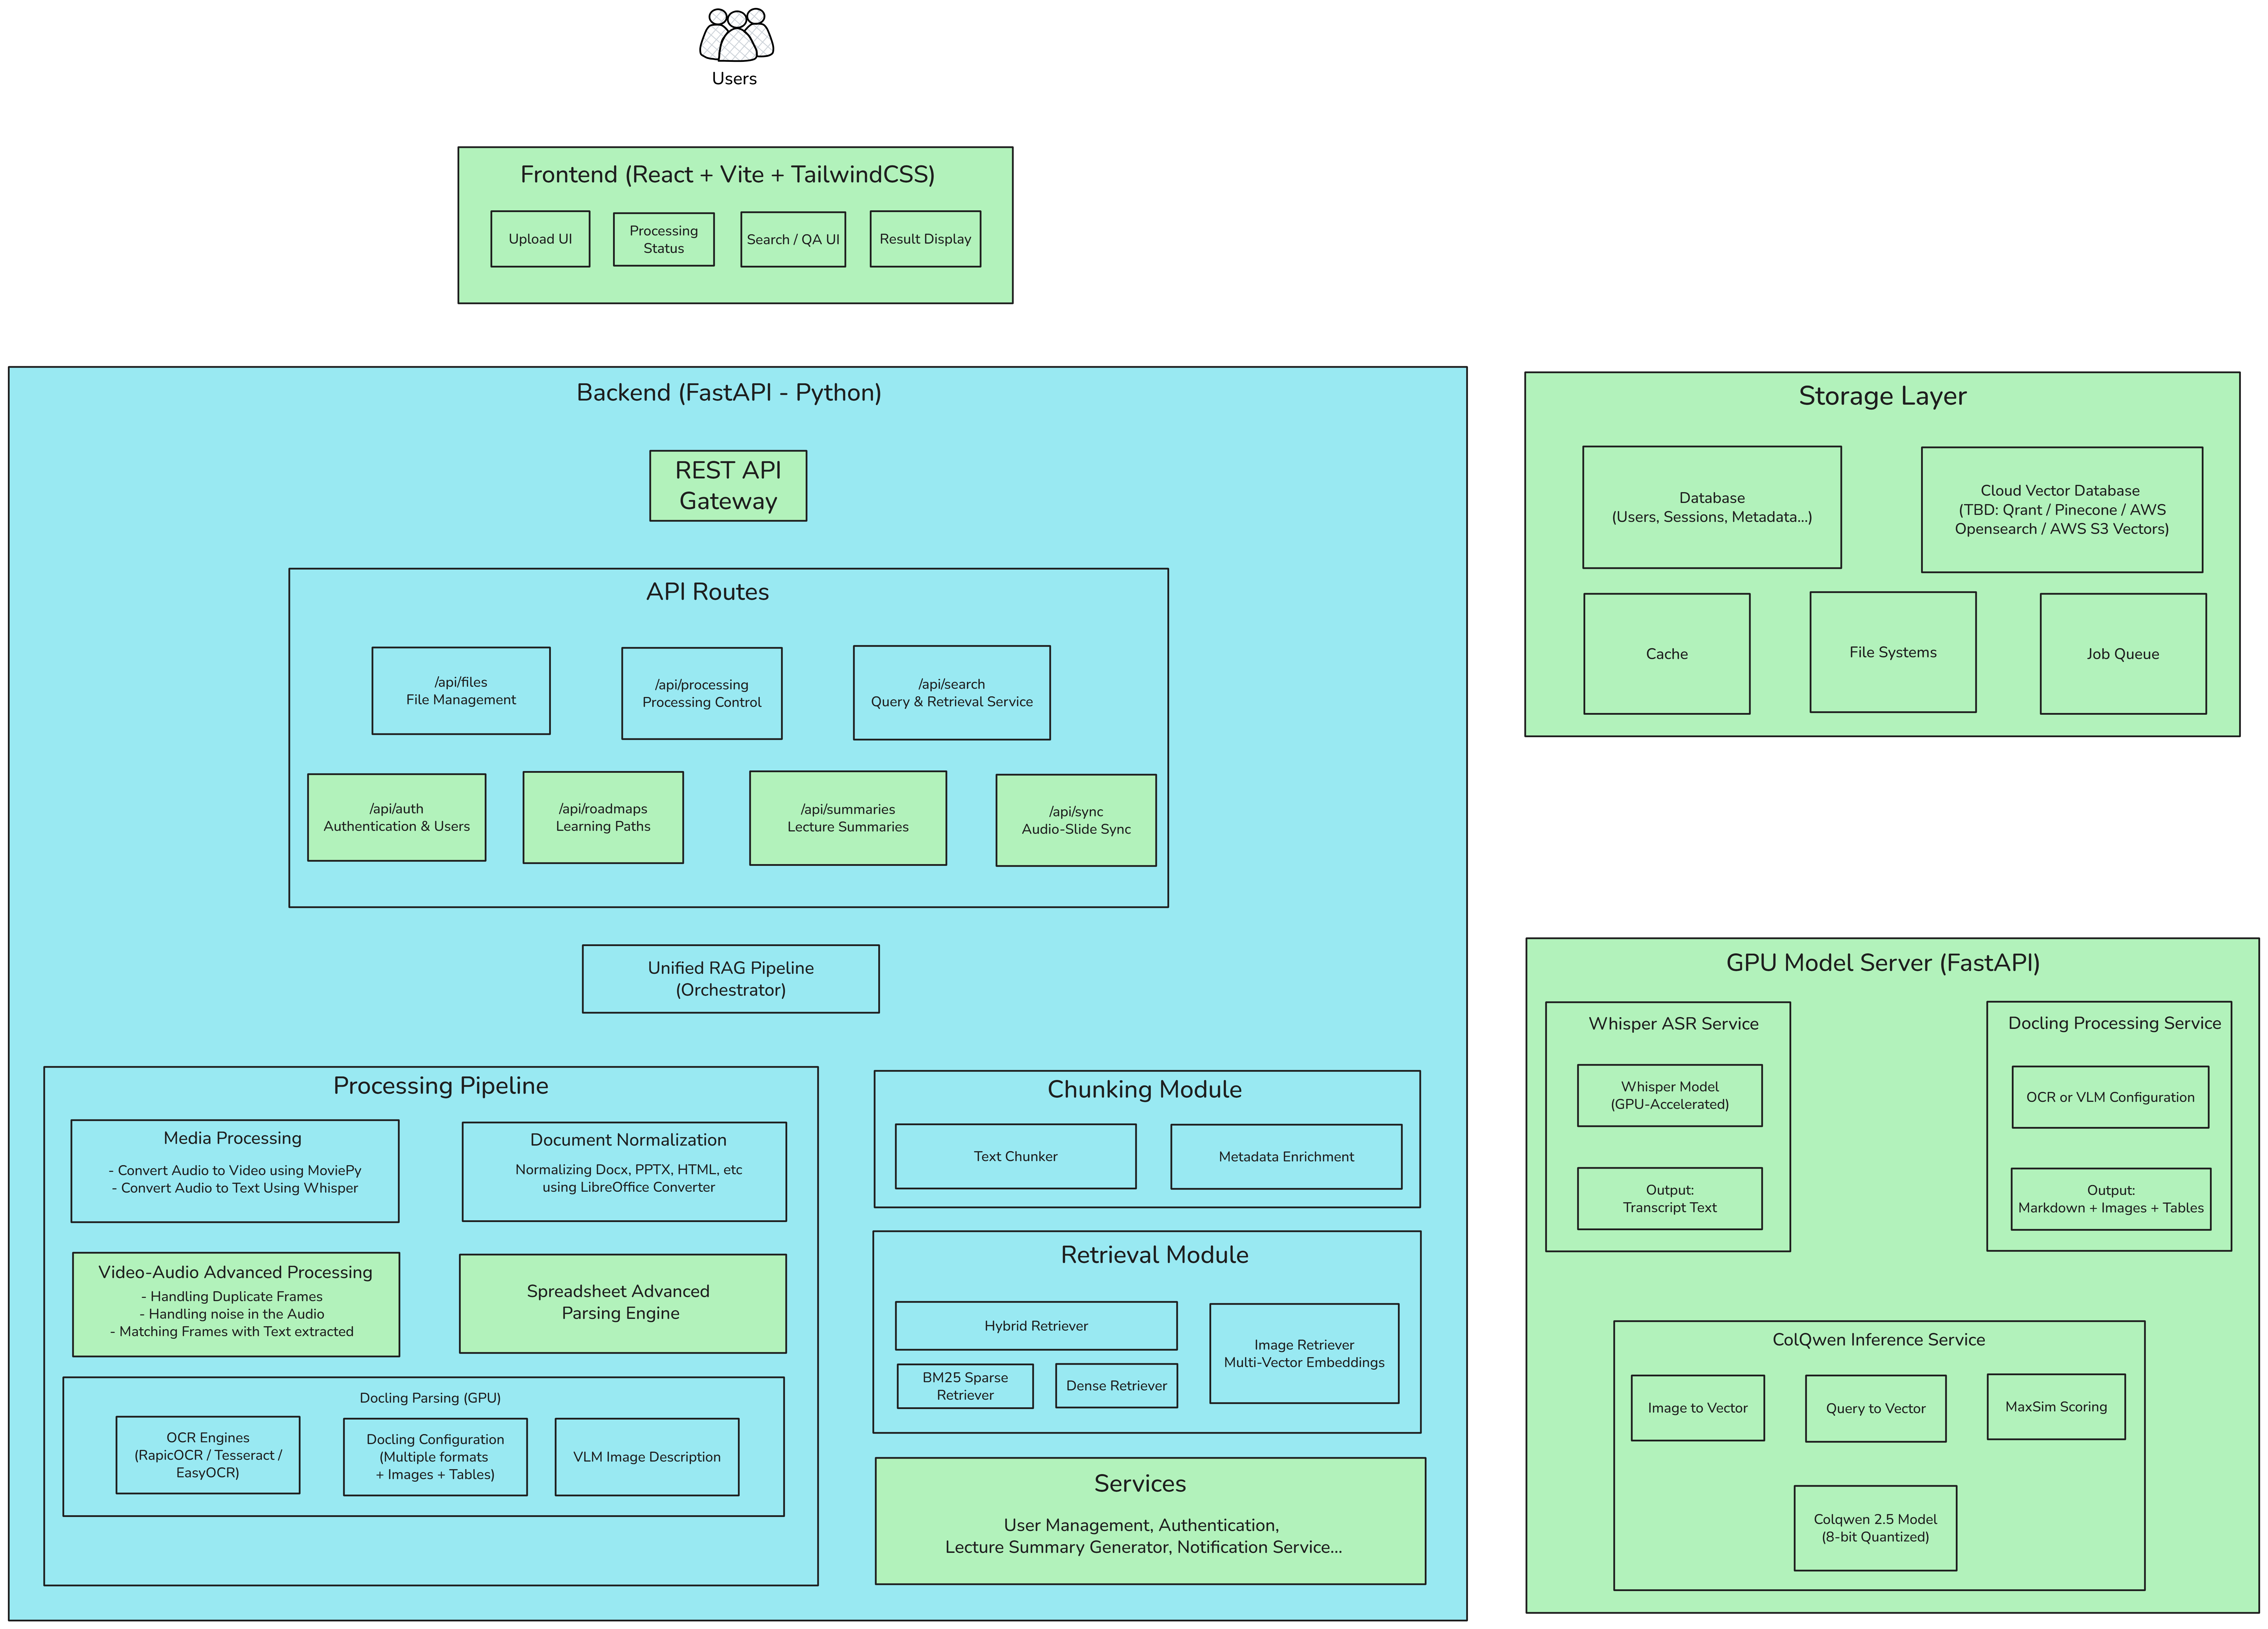
\includegraphics[width=\textwidth]{img/pdz/excalidraw-architecture.png}
    \caption{BK-MInD High-Level System Architecture.}
    \label{fig:high_level_arch}
\end{figure}

The BK-MInD system architecture, illustrated in Figure~\ref{fig:high_level_arch}, is organized into four interconnected layers that span from the user interface to the underlying cloud infrastructure.

The \textbf{Interface Layer} comprises the React-based frontend, which provides dedicated views for document upload, pipeline monitoring, knowledge exploration, learning roadmap generation, quiz creation, and an interactive chat assistant. All user interactions are routed through a single-page application that communicates with the backend exclusively via REST API calls.

The \textbf{API and Orchestration Layer} is implemented using FastAPI and acts as the central controller of the system. It exposes asynchronous endpoints for document ingestion, pipeline triggering, index construction, and query processing. The \texttt{UnifiedRAGPipeline} orchestrator coordinates all processing stages and maintains system state through Amazon DynamoDB, while task queues managed by Amazon SQS decouple long-running pipeline jobs from synchronous API responses.

The \textbf{Data Processing and Indexing Layer} implements the 7-stage conditional pipeline (detailed in Section~\ref{sec:pipeline_arch}) that transforms raw educational materials — PDFs, DOCX, PPTX, Excel spreadsheets, audio, and video — into RAG-ready artifacts. Following processing, the dual-pathway embedding module produces both text indices (BM25, dense FAISS, and hybrid) and visual indices (ColQwen multi-vector embeddings) stored in Qdrant Cloud.

The \textbf{Cloud Infrastructure Layer} leverages Amazon Web Services for scalable deployment. Amazon S3 provides persistent object storage for all document artifacts; EC2 Auto Scaling groups host computationally intensive inference services (Whisper ASR and ColQwen visual embeddings); and Amazon ECS Fargate runs the containerized frontend and backend services. Amazon CloudFront and AWS WAF form the ingress tier, providing CDN acceleration and edge-level security filtering. Together, these four layers enable BK-MInD to ingest diverse HCMUT lecture materials, build a multimodal knowledge index, and serve interactive educational features.

\subsection{Pipeline Architecture}\label{sec:pipeline_arch}

The system implements a dual-pipeline architecture designed to handle heterogeneous document formats and produce RAG-ready outputs for both text-based and image-based retrieval. The architecture is divided into two primary pipelines: the Data Processing Pipeline and the Embedding-Indexing Pipeline.

\textbf{Data Processing Pipeline}

\begin{figure}[h!]
    \centering
    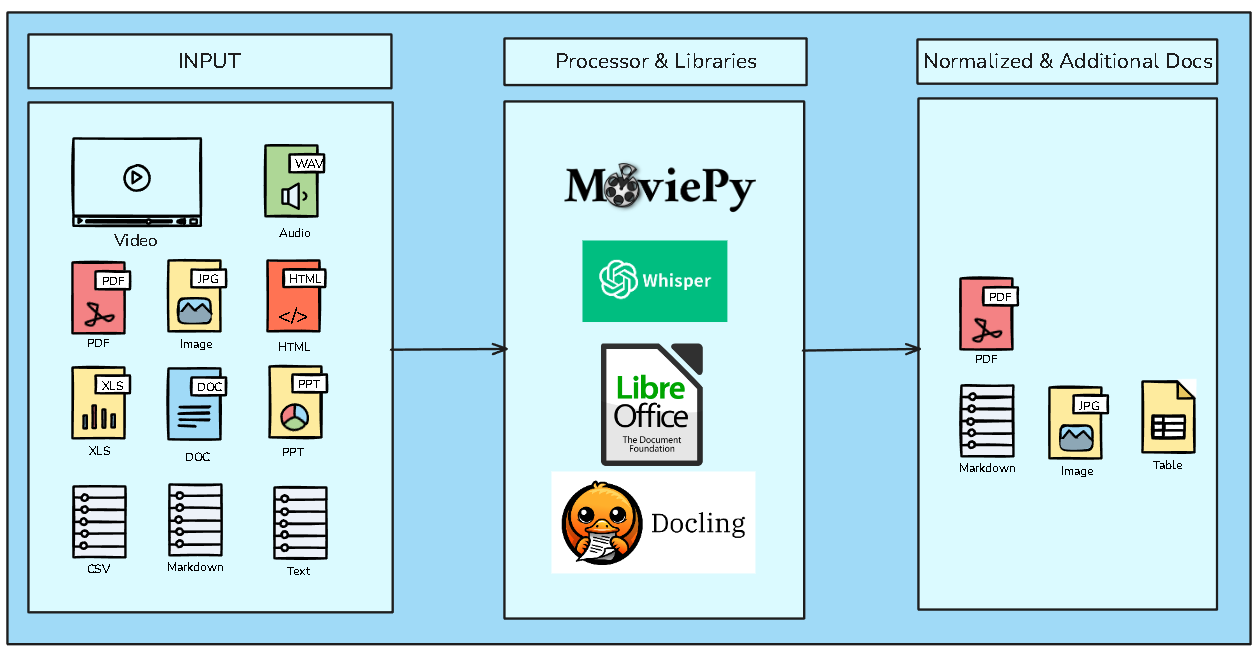
\includegraphics[width=\textwidth]{img/pdz/19-normalization.png}
    \caption{Data Processing Pipeline Normalization Stage.}
    \label{fig:normalization}
\end{figure}

The MRAG system implements a \textbf{7-stage conditional processing pipeline} that transforms diverse input formats into RAG-ready artifacts. As illustrated in Figure~\ref{fig:normalization}, the pipeline routes documents through format-specific processors only when needed, optimizing resource utilization while preserving semantic structure. The pipeline is designed around three key principles:

\begin{enumerate}
    \item \textbf{Format-Specific Optimization}: Different document formats (Excel, DOCX, PDF) contain structural information (tables, heading hierarchies, page boundaries) that generic parsers miss. Custom parsers in Stages 3b, 3c, and 3d preserve this structure, yielding higher-quality chunks for retrieval.

    \item \textbf{Conditional Routing}: Not all documents require all stages. By implementing conditional execution, the system processes only what is necessary. A plain text file skips Stages 3b/3c/3d entirely, while an Excel spreadsheet runs the specialized Stage 3b parser. This design minimizes wasted computation.

    \item \textbf{Multimodal Fusion}: Stage 2 extracts multimedia content (audio transcripts, video frames) that Stage 3 cannot handle. Stage 4 consolidates all outputs — text from all sources, images from document pages and extracted diagrams, and transcripts from media — into a unified, retrievable index.
\end{enumerate}

\begin{table}[H]
\centering
\caption{7-Stage Pipeline Summary}
\label{tab:7stage_quick}
\scalebox{0.8}{
\begin{tabular}{llp{6cm}l}
\toprule
\textbf{Stage} & \textbf{Name} & \textbf{Role} & \textbf{Execution} \\ \midrule
1 & Normalization & Format detection and routing & Always \\
2 & Media Processing & Audio/video extraction and transcription & Conditional \\
3 & Main Document Processing & Structural analysis via Docling & Always \\
3b & Excel Processing & Table-aware custom parsing & Conditional \\
3c & DOCX Processing & Heading-aware custom parsing & Conditional \\
3d & PDF Processing & Born-digital document parsing & Conditional \\
4 & Consolidation & Merge all outputs, prepare for indexing & Always \\ \bottomrule
\end{tabular}
}
\end{table}

For detailed specifications of each stage including routing tables, processing parameters, and output structures, refer to Chapter~6 (Implementation).

\textbf{Embedding-Indexing Pipeline}

\begin{figure}[h!]
    \centering
    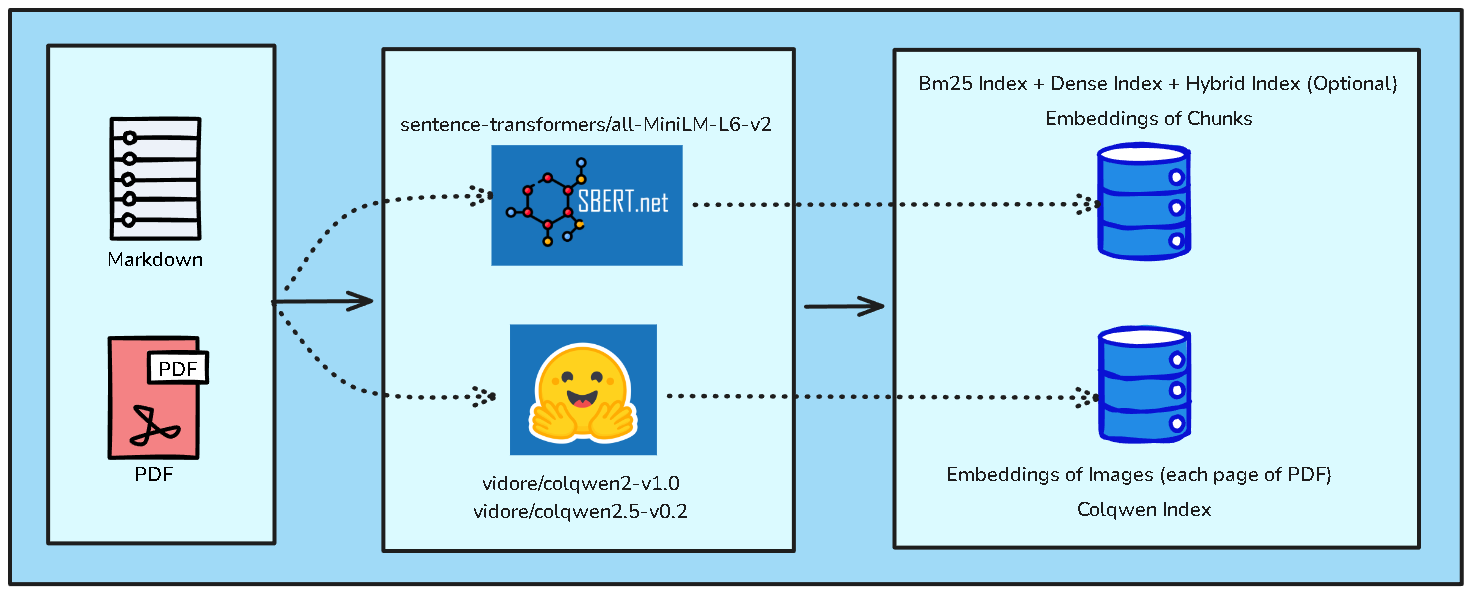
\includegraphics[width=\textwidth]{img/pdz/27-chunkemb.png}
    \caption{Dual-Pathway Embedding and Indexing Architecture.}
    \label{fig:chunk_emb}
\end{figure}

Following data processing, the system employs a dual-pathway embedding architecture to enable multimodal retrieval. As illustrated in Figure~\ref{fig:chunk_emb}, this architecture allows simultaneous retrieval of granular text segments and holistic document pages.

\textit{Text Embedding Pathway}: Structured Markdown files are segmented using \texttt{RecursiveCharacterTextSplitter} (1024-character chunks, 200-character overlap) and encoded into 384-dimensional vectors by \texttt{all-MiniLM-L6-v2}. The system maintains three parallel indices: a BM25 inverted index for keyword retrieval, a FAISS dense index for semantic search, and a hybrid index combining both via Reciprocal Rank Fusion (RRF).

\textit{Visual Embedding Pathway}: PDF pages are rasterized at 150 DPI using a ``1 Page = 1 Image'' strategy. Each page image is processed by ColQwen2, a Vision-Language Model using the Late Interaction paradigm, generating multi-vector patch-level embeddings stored in the ColQwen visual index. This enables diagram-aware and layout-aware retrieval without relying on OCR.

\textbf{Pipeline Output Summary}

The complete pipeline produces the following RAG-ready artifacts:

\begin{itemize}
    \item \textbf{Text-Based Retrieval}: Markdown files with three indices (BM25, Dense, Hybrid) enabling keyword and semantic search over chunked content.
    \item \textbf{Image-Based Retrieval}: Rasterized PDF pages with ColQwen visual embeddings enabling layout-aware and diagram-sensitive search.
    \item \textbf{Structured Data}: Extracted tables (CSV + Markdown), isolated images, and comprehensive metadata (JSON) for provenance tracking.
    \item \textbf{Multimedia Transcripts}: Time-stamped text transcriptions from video/audio in multiple formats (TXT, JSON, SRT, VTT).
\end{itemize}

\subsection{Retrieval and Generation Flow}

\begin{figure}[h!]
    \centering
    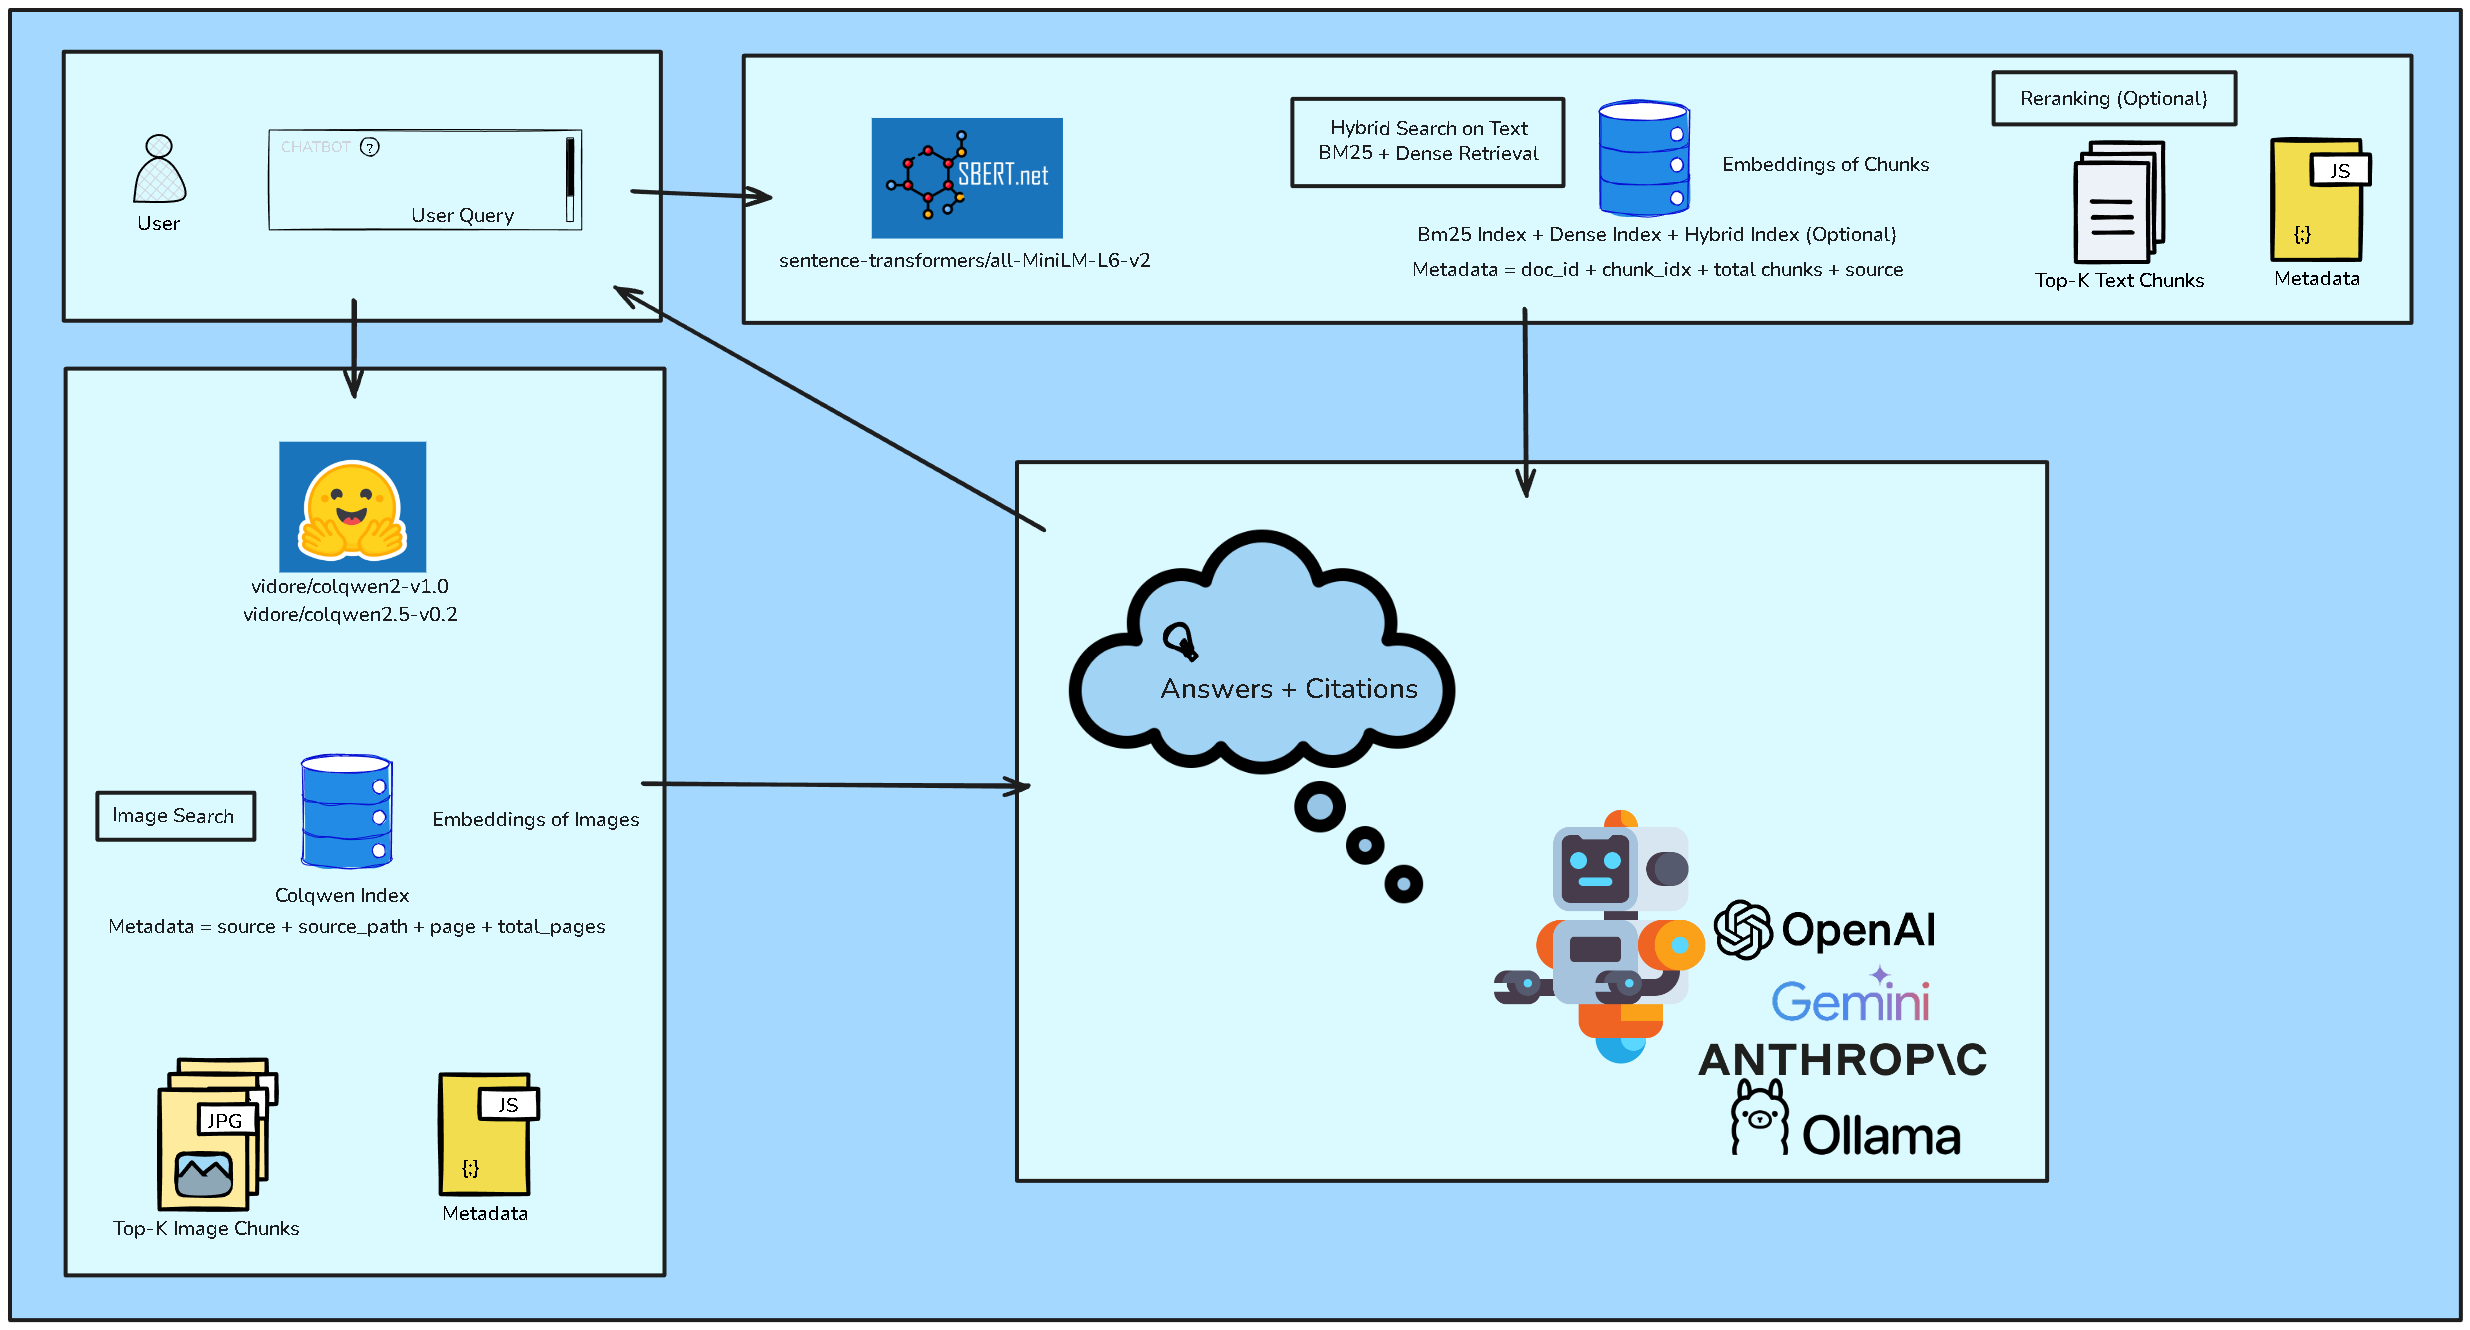
\includegraphics[width=1\textwidth]{img/pdz/22-architecture.png}
    \caption{Overall MRAG System Architecture: Retrieval and Generation Flow.}
    \label{fig:overall_arch}
\end{figure}

When a user submits a query to the system, it triggers a parallel retrieval pipeline designed to gather both textual and visual evidence in support of answer generation. The complete flow is illustrated in Figure~\ref{fig:overall_arch}.

\textbf{Query Processing Pipeline}

The query processing flow follows this sequence:

\begin{enumerate}
    \item \textbf{Query Input}: User submits a natural language question via the chat interface.
    \item \textbf{Parallel Encoding}: The query is simultaneously encoded by two engines:
    \begin{itemize}
        \item \textbf{Text Encoder}: Encodes the query into a 384-dimensional dense vector using the same model as the corpus (all-MiniLM-L6-v2).
        \item \textbf{Visual Encoder}: Encodes the query using ColQwen's query encoder to prepare for late-interaction visual matching.
    \end{itemize}
    \item \textbf{Parallel Retrieval}: Both streams search their respective indices independently.
    \item \textbf{Context Aggregation}: Top-K results from each stream are merged into a unified context.
    \item \textbf{Just-in-Time Rendering}: Retrieved PDF pages are rendered to high-resolution images on-demand.
    \item \textbf{LLM Generation}: The aggregated context is passed to the LLM for answer synthesis.
\end{enumerate}

\textbf{Text Retrieval Options}

The system offers three complementary text retrieval strategies, each addressing different query characteristics:

\textit{1. Sparse (BM25) Retrieval}: BM25 is a probabilistic ranking function based on term frequency and inverse document frequency. It excels when queries contain specific keywords, entity names, or exact phrases. Strengths include robust exact term matching; weakness is failure on semantic paraphrases.

\textit{2. Dense (Embedding-Based) Retrieval}: Dense retrieval encodes both queries and documents as continuous vectors in a high-dimensional space. It captures semantic meaning and handles paraphrased queries effectively, though it is susceptible to ``semantic drift'' — retrieving documents that are topically similar but factually incorrect.

\textit{3. Hybrid Retrieval (BM25 + Dense + RRF)}: The system implements \textbf{Reciprocal Rank Fusion (RRF)}, a fusion algorithm that combines BM25 and dense retrieval results. For each document, RRF calculates:

\[
\text{RRF}(d) = \frac{1}{k + \text{rank\_BM25}(d)} + \frac{1}{k + \text{rank\_Dense}(d)}
\]

where $k$ is a constant (typically 60) that smooths the contribution of both rankers. Hybrid retrieval is the \textbf{default strategy} for all queries, balancing keyword precision with semantic understanding.

\textbf{Visual Retrieval}

In parallel with text retrieval, the system searches for relevant document pages using visual embeddings. ColQwen's late-interaction architecture allows the system to match query concepts against the visual structure of pages, retrieving diagrams, charts, and tables that may not be adequately represented in extracted text.

\begin{itemize}
    \item \textbf{Query Encoding}: The query is encoded by ColQwen's text encoder into a set of multi-vector embeddings.
    \item \textbf{Page Matching}: These vectors are matched against stored page embeddings using MaxSim scoring, identifying pages with visually relevant content.
    \item \textbf{Just-in-Time Rendering}: Retrieved pages are rendered to JPEG images and passed to the multimodal LLM, enabling it to ``see'' charts, graphs, and layout-dependent information.
\end{itemize}

\textbf{Reranking and Design Decision}

\textit{Current Implementation}: Reranking is \textbf{globally disabled} in production (\texttt{skip\_reranker=true}) for latency optimization. Cross-encoder reranking adds 1-2 minutes of latency, making it unsuitable for interactive chat applications.

\textit{Historical Context}: During Phase 1 evaluation, cross-encoder reranking (using BGE-Large) improved nDCG@3 from 0.8855 (dense alone) to 0.9248, demonstrating significant accuracy gains. However, this comes at the cost of $\sim$100x latency increase.

\textit{Current Approach}: Hybrid retrieval via RRF provides a strong balance of accuracy and latency without reranking. The reranker code is retained in the codebase for fast rollback if future evaluation shows reranking benefits justify the latency trade-off.

\textbf{Context Aggregation and Generation}

After retrieval, the system aggregates top-K text chunks and top-K visual pages into a unified context window:

\begin{enumerate}
    \item \textbf{Text Context}: Top-K text chunks from hybrid retrieval are concatenated with their metadata (source, page number, heading).
    \item \textbf{Visual Context}: Top-K pages are rendered to high-resolution JPEG images.
    \item \textbf{Context Size}: The total context is sized to fit within the LLM's context window (typically 16k-32k tokens, depending on the model).
    \item \textbf{LLM Selection}: The system supports multiple LLM providers (OpenAI GPT-4o, Anthropic Claude, Google Gemini, or local models via Ollama).
\end{enumerate}

The LLM reads this aggregated context and generates a natural language answer grounded in the retrieved evidence. Importantly, the LLM includes precise citations — linking every factual claim to the specific chunk or page from which it was derived. This ensures traceability and enables users to verify the system's reasoning.

\subsection{Security Architecture}\label{sec:security_arch}

\begin{figure}[h!]
    \centering
    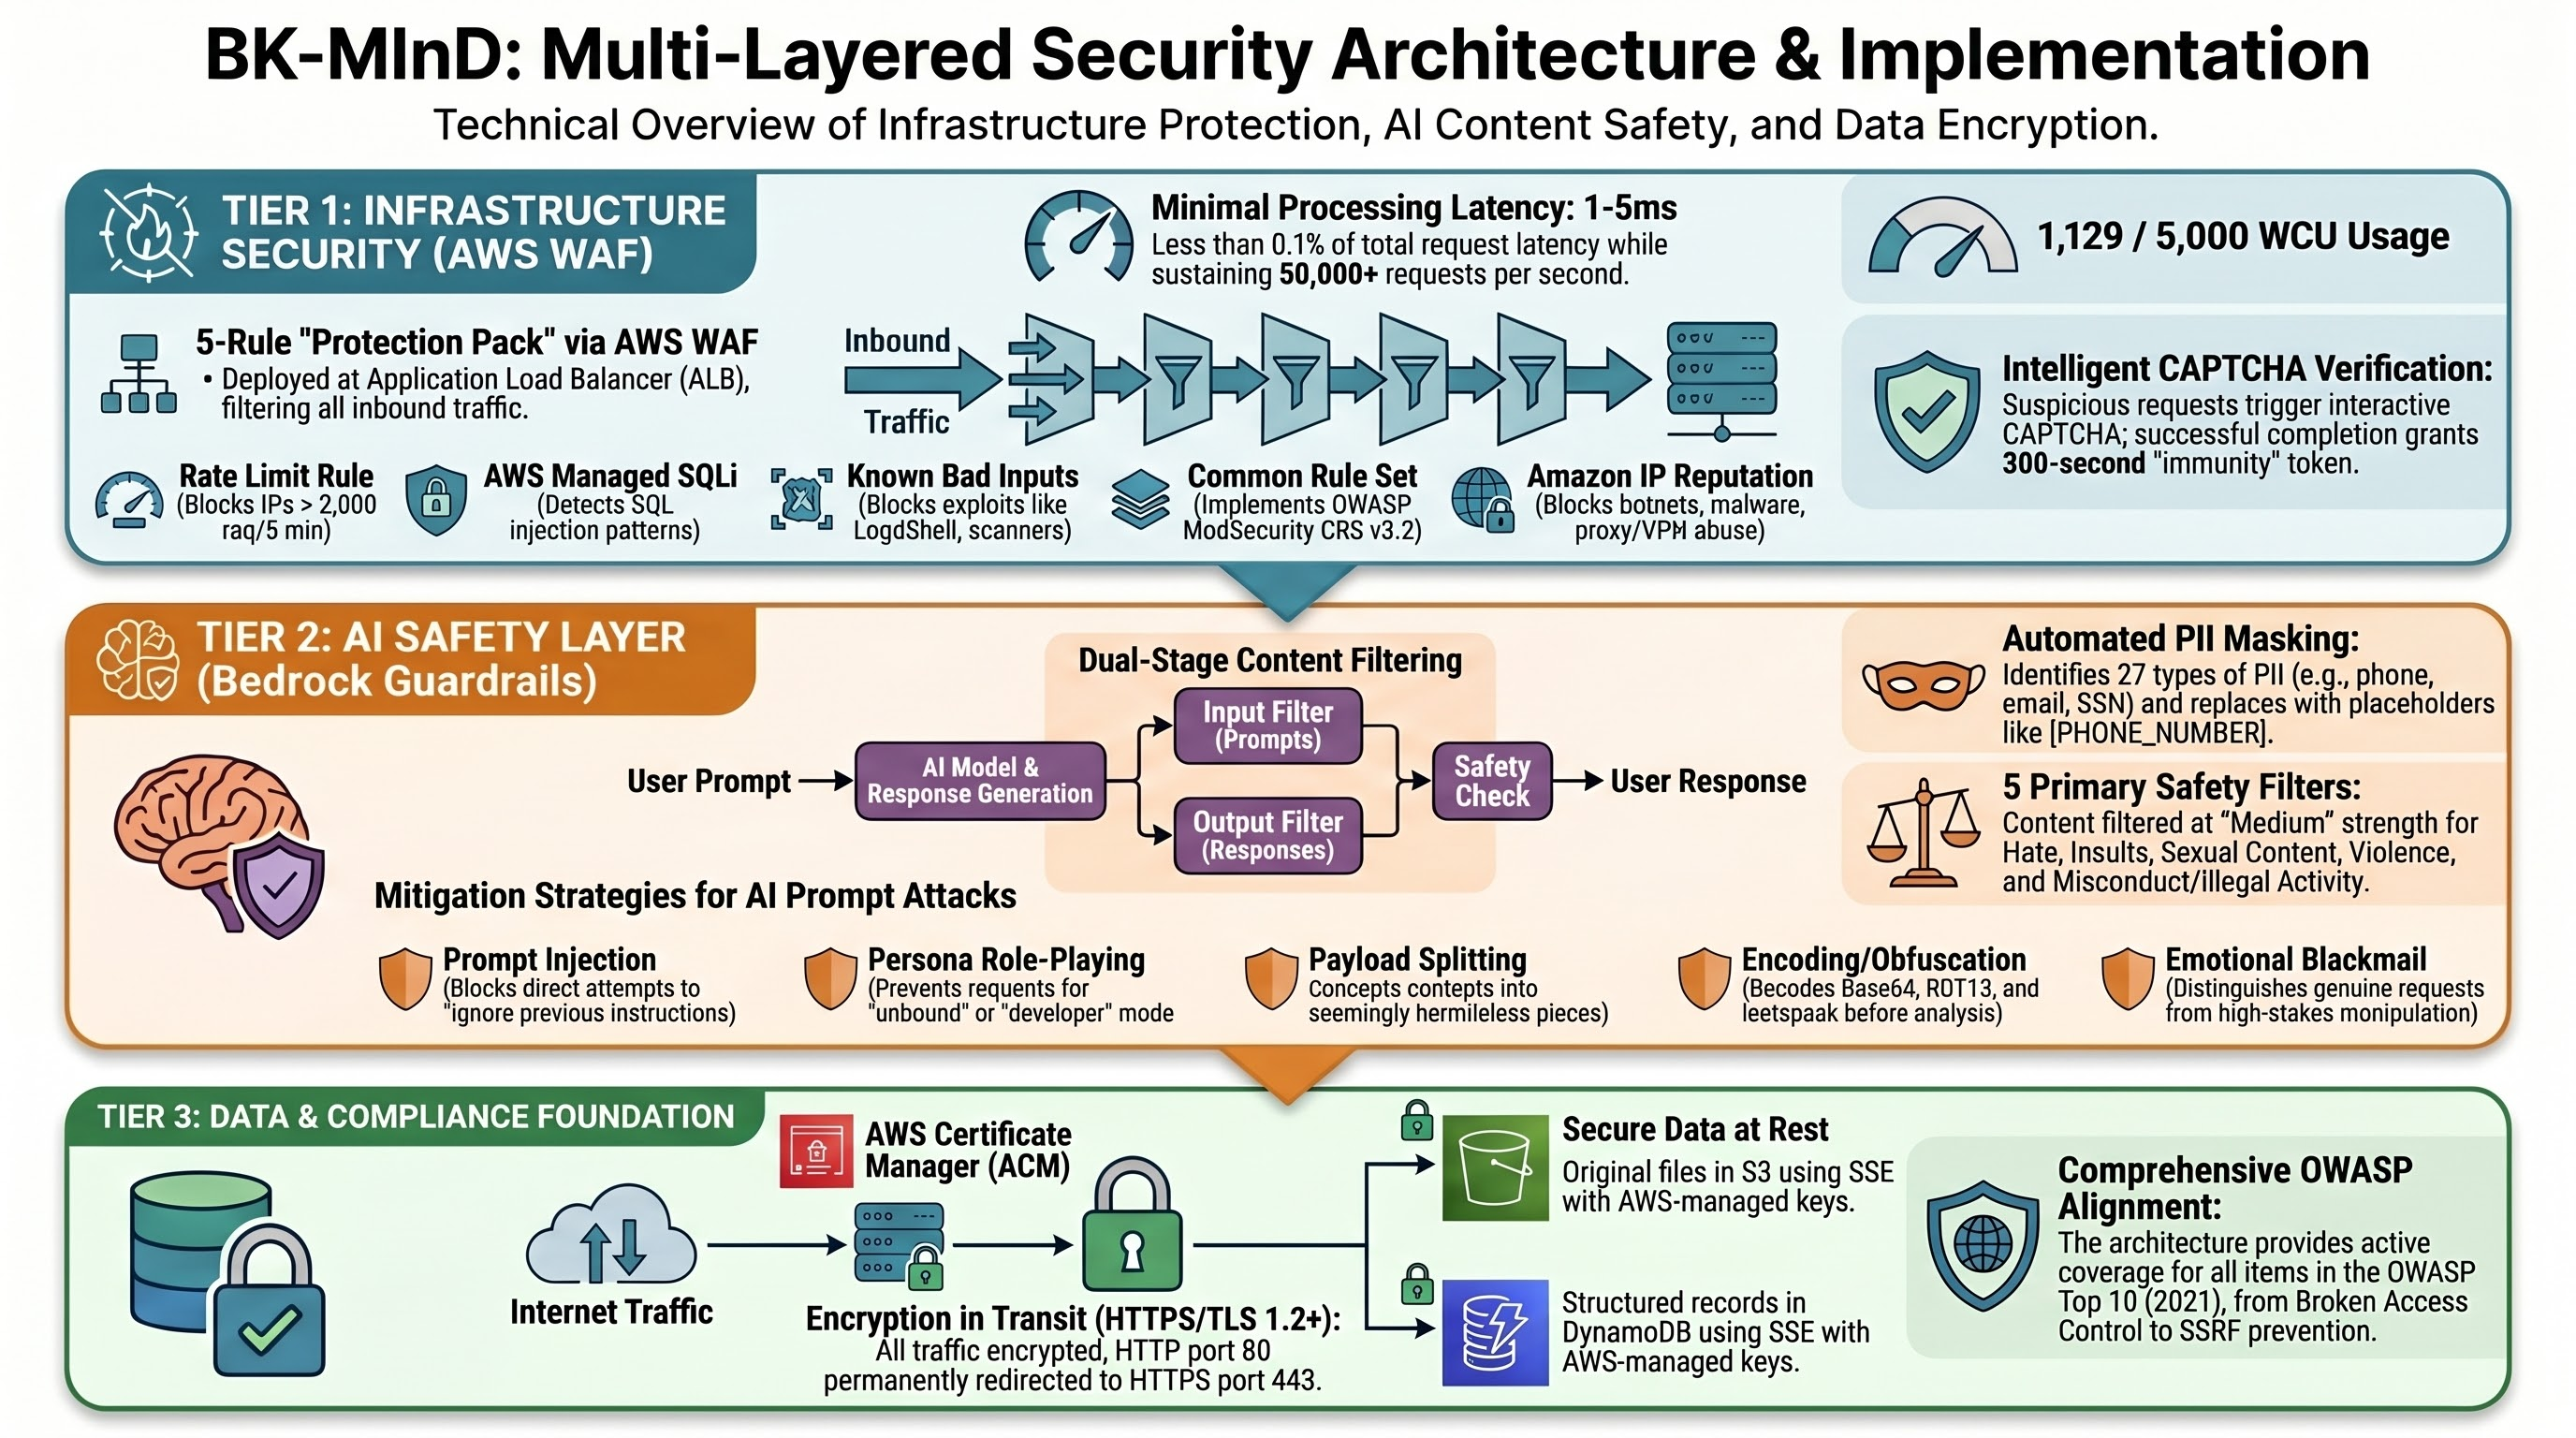
\includegraphics[width=\textwidth]{img/pdz/49-security-arch.jpg}
    \caption{BK-MInD Three-Tier Security Architecture.}
    \label{fig:security_arch}
\end{figure}

The BK-MInD system implements a three-tier security architecture, as illustrated in Figure~\ref{fig:security_arch}, that protects the system at the network edge, application logic, and data storage levels. Implementation details and specific configuration parameters for each component are documented in Chapter~6 (Implementation).

\textbf{Tier 1 — Network Edge Protection (AWS WAF)}: All incoming traffic passes through an AWS Web Application Firewall configured with a five-rule protection pack. The rules enforce protection against SQL injection, cross-site scripting (XSS), HTTP flood attacks (rate limiting), geographic access control, and automated bot filtering. This layer ensures that malicious requests are rejected before reaching the application servers.

\textbf{Tier 2 — Application-Layer Content Filtering (Bedrock Guardrails)}: The LLM generation pipeline integrates Amazon Bedrock Guardrails as a dual-stage content filter applied to both user inputs and model outputs. The guardrails enforce topic restrictions (preventing off-topic misuse), apply personally identifiable information (PII) masking to anonymize sensitive data, and block toxic or harmful content categories. This ensures that the educational assistant remains on-topic and appropriate for academic contexts.

\textbf{Tier 3 — Data Encryption and Transmission Security}: All data in transit is protected by TLS/HTTPS enforced through AWS Certificate Manager (ACM)-issued certificates. Data at rest in Amazon S3 is encrypted using server-side encryption (SSE). The API communication between frontend and backend is further secured through JWT-based authentication tokens, ensuring that only authorized users can access document repositories and generation features.

The experimental findings above directly inform the hardware and software specifications required to reliably operate the BK-MInD system at production scale. Based on the observed latency and resource consumption patterns during evaluation, the following section specifies the minimum and recommended computational requirements.

\section{Technical Requirements}

\subsection{Hardware Requirements}

\begin{itemize}
    \item \textbf{GPU}: NVIDIA GPU with at least 4GB of VRAM, but when using 8GB VRAM, we recommend (RTX 4060, RTX 4070, or equivalent) for efficient embedding generation and inference. For larger models or batch processing, 16GB+ VRAM is recommended.
    \item \textbf{CPU}: Multi-core processor (8+ cores) to support parallel processing of documents and concurrent API requests.
    \item \textbf{Memory (RAM)}: Minimum 16GB of system RAM for running the entire pipeline, including model caching and document processing.
\end{itemize}

\subsection{Software Dependencies}

\begin{itemize}
    \item \textbf{Core Frameworks}:
    \begin{itemize}
        \item \textbf{Frontend}: React 19 with Tailwind 4.1 for high-performance UI components.
        \item \textbf{Backend}: FastAPI for the asynchronous REST API framework.
        \item \textbf{Database}: Qdrant Cloud for vector storage with payload isolation; Amazon DynamoDB for chat persistence.
    \end{itemize}
    \item \textbf{AI Processing Engines}:
    \begin{itemize}
        \item \textbf{Docling}: Document understanding framework for structural analysis.
        \item \textbf{Whisper Large-v3}: High-fidelity ASR for multi-language transcription.
        \item \textbf{SmolVLM-256M}: Optional lightweight Vision-Language Model for page layout understanding in Docling. When enabled in configuration, SmolVLM-256M (256M parameters) provides an OCR-alternative approach for document parsing with lower latency than larger VLMs, trading some extraction quality for faster processing speed. Particularly useful for rapid prototyping and latency-constrained deployments.
        \item \textbf{ColQwen2.5-v1.0}: Late-interaction visual retrieval engine.
    \end{itemize}
    \item \textbf{Model Weights}:
    \begin{itemize}
        \item \texttt{all-MiniLM-L6-v2} (Standard) or \texttt{BGE-M3} (Advanced) for text embeddings.
        \item \texttt{bge-reranker-large} for optional reranking (currently globally disabled for latency optimization).
        \item LLM backbone: Supporting Claude 3.5 Sonnet (via Bedrock) or GPT-4o.
    \end{itemize}
\end{itemize}

\subsection{System Architecture Constraints}

\textbf{Advantages:}
\begin{itemize}
    \item \textbf{Data Security and Privacy}: Document artifacts and processing pipelines are deployed on AWS infrastructure with multi-layered encryption. Document storage uses Amazon S3 with server-side encryption (SSE) enabled by default and access control via IAM policies. All data in transit is protected by TLS 1.3/HTTPS enforced through AWS Certificate Manager (ACM)-issued certificates. Multi-tenant isolation is enforced through S3 key prefixing by user ID and DynamoDB partition isolation, preventing cross-user data leakage and ensuring compliance with HCMUT data governance policies.
    \item \textbf{Concurrency}: The system is designed to handle multiple concurrent API requests using FastAPI's asynchronous architecture, supporting up to $N$ simultaneous users (where $N$ is bounded by available memory and GPU scheduling).
    \item \textbf{Scalability}: The modular pipeline design allows for independent scaling of retrieval and generation components. Additional indexing nodes can be added for large document corpora without modifying the core system.
    \item \textbf{Portability}: The entire system can be containerized using Docker, enabling seamless deployment across different environments (development, staging, production).
\end{itemize}

\textbf{Limitations:}
\begin{itemize}
    \item \textbf{Single-GPU Dependency}: The current architecture does not support distributed GPU processing. Visual embedding generation (ColQwen) and inference are constrained to a single GPU, creating a bottleneck for large-scale batch processing.
    \item \textbf{Index Rebuilding Overhead}: Document updates require full index regeneration. The system does not support incremental indexing, meaning that adding or modifying a single document necessitates reprocessing the entire corpus for that index type.
    \item \textbf{Memory Scalability}: Both BM25 and FAISS indices are loaded entirely into RAM during retrieval. For corpora exceeding 1 million documents, memory consumption can surpass 32GB, limiting deployment on consumer-grade hardware.
    \item \textbf{Storage Redundancy}: The dual-pathway architecture stores multiple representations of the same document (original PDF, rasterized images, Markdown, embeddings), resulting in storage overhead of approximately $5\times$ the original document size.
    \item \textbf{Processing Latency}: Document ingestion is synchronous and blocking. A single complex PDF (e.g., 100 pages with tables and images) can take 2-5 minutes to process through the full pipeline, during which no other documents can be processed concurrently.
    \item \textbf{Model Size Constraints}: The system's embedding models are fixed at deployment time. Switching to larger models (e.g., upgrading from MiniLM to BGE-Large for embedding) requires reindexing the entire corpus. Reranking is globally disabled by default (\texttt{skip\_reranker=true}) for latency optimization, though the code is retained for fast rollback.
    \item \textbf{Limited Multi-Tenancy}: The file-system-based storage architecture lacks built-in isolation mechanisms. Deploying the system for multiple independent clients requires separate instances or manual namespace management.
\end{itemize}
